% -----------------------------------------------------------------------------
\begin{frame}[c]
\frametitle{Predictive control, operating WWTPs as self-sufficient WRRFs} \justifying

\boxHighlight[0.95\textwidth]{ \centering
    \textbf{Paradigm shift:} Wastewater as a sustainable source of water, energy, and raw materials
}

\vfill

\begin{center}
    \includegraphics<1>[width=0.95\textwidth]{figs/ControlFramework_01}%
    \includegraphics<2>[width=0.95\textwidth]{figs/ControlFramework_02}%
\end{center}

\vfill

\onslide<2>{
\boxInfo[0.95\textwidth]{\centering
    \textbf{Proposal (A):} Predictive control to enable self-sufficient water resource recovery facilities
}
}

\end{frame}

% -----------------------------------------------------------------------------
\section{(Proposal A)\\Predictive control for transitioning WWTPs\\ into self-sufficient WRRFs} \sectioncover
% -----------------------------------------------------------------------------
\begin{frame}[c]
\frametitle{Predictive control, operating WWTPs as self-sufficient WRRFs} \justifying

\vskip1em

\boxHighlight[0.9\textwidth]{ \centering
    We consider the task of operating a \textbf{biological wastewater treatment plant} (WWTP, secondary treatment) as a \textbf{water resource recovery facility} (WRRF)
}

\vfill

\begin{center}
    \includegraphics<1>[width=0.95\textwidth]{figs/ControlFramework_01}%
    \includegraphics<2>[width=0.95\textwidth]{figs/ControlFramework_02}%
\end{center}

\vfill

\end{frame}


% -----------------------------------------------------------------------------
\begin{frame}[t]
\frametitle{Predictive control, operating WWTPs as self-sufficient WRRFs (cont.)}\justifying
	
\vskip1em

\boxHighlight[0.9\textwidth]{ \centering
    We consider the task of operating a \textbf{biological wastewater treatment plant} (WWTP, secondary treatment) as a \textbf{water resource recovery facility} (WRRF)
}

\vfill

\begin{columns}
	\column[c]{0.45\textwidth}%
	\includegraphics[width=\columnwidth]{figs/WRRF_Schematic_Instrumented_Colors}

	\column[c]{0.54\textwidth}
	\begin{itemize}
		\item {\color{monokaiOrange}\sc Primary objective:}\\
		on demand, produce effluent water of specific quality
		\vskip0.5em
		\begin{center}
            \begin{tabular}{@{}c ccc@{}} \toprule
                Water class & \multicolumn{3}{c}{Biochemical profile}                   \\\midrule
                            & {\small TSS}      &    {\small BOD}   &    {\small  TN}   \\\cmidrule{2-4}
                \textbf{A}  & $\leq 30$ g/m$^3$ & $\leq 10$ g/m$^3$ & $\leq 15$ g/m$^3$ \\
                \textbf{B}  & $\leq 30$ g/m$^3$ & $\leq 15$ g/m$^3$ & $\leq 30$ g/m$^3$ \\
                \textbf{C}  & $\leq 30$ g/m$^3$ & $\leq 20$ g/m$^3$ & $\leq 45$ g/m$^3$ \\\bottomrule
            \end{tabular}
		\end{center}
		\vskip1.5em
		%
		\item {\color{monokaiOrange}\sc Secondary objective:}\\
		produce biogas to ensure nonpositive energy cost index,
		\begin{multline*}
			\text{ECI} = \text{AE} + \text{PE} + \text{ME} - \eta_{E} \text{MP} \\
                            + \max(0, \text{HE} - \eta_{H}\text{MP})
		\end{multline*}
	\end{itemize}
\end{columns}

\vfill

\end{frame}

%------------------------------------------------------- 
\begin{frame}[t]
\frametitle{Predictive control, general architecture and specific configuration}\justifying

\vskip0.66em

\begin{columns}
	\column[t]{0.5\textwidth}
	\begin{center}
		\vskip-1.5em
		\includegraphics<1>[width=0.98\columnwidth]{figs/Control_Diagram_Isolated}% 
		\includegraphics<2>[width=0.98\columnwidth]{figs/Control_Diagram_Isolated_H1}% 
		\includegraphics<3>[width=0.98\columnwidth]{figs/Control_Diagram_Isolated_H2}% 
		\includegraphics<4>[width=0.98\columnwidth]{figs/Control_Diagram_Isolated_H3}% 
	\end{center}

	\column[t]{0.49\textwidth}
	We design a \textbf{model-based} output-feedback controller
    \begin{equation*}
        \Sigma \coloneqq \left\{
            \begin{aligned}
                \textstyle\frac{d}{dt}\clX{x(t)} &= f(\clX{x(t)}, \clW{w(t)}, \clU{u(t)})   & \text{\footnotesize\color{gray}(dynamics)} \\
                \clY{y(t)}   				     &= g(\clX{x(t)}, \clW{w(t)}, \clU{u(t)})   & \text{\footnotesize\color{gray}(measurements)} \\
                \clY{z(t)}   				     &= h(\clX{x(t)}, \clW{w(t)}, \clU{u(t)})   & \text{\footnotesize\color{gray}(performance)}
            \end{aligned}
        \right.
    \end{equation*}

	\vskip0.5em
	which autonomously operates the plant in cycles	
	\begin{center}
		\includegraphics[width=0.9\columnwidth]{figs/Control_Diagram_Time}
	\end{center}
\end{columns}

\vskip2em

\only<2>{\centering%
\begin{minipage}{0.99\textwidth} \centering
    \textsc{\color{monokaiOrange}OPO:} Obtains a linearization of $\Sigma$ centered on a \emph{operating point} producing the \emph{desired KPIs}
    \vskip-0.5em
	\begin{block}{} \centering
    \begin{columns}
        \column[c]{0.45\columnwidth}
        \vskip-2em
		\begin{align*}
            \underset{x_k,~ u_k}{\text{minimize}} \quad
            & \left\| 
                    \clP{\begin{bmatrix} W_{z|\text{ref}} & \\ & W_{u|\text{ref}} \end{bmatrix} }
                    \begin{bmatrix} 
                        \clY{z_k - \bar{z}^{\text{ref}}_k} \\ 
                        \clU{u_k - \bar{u}^{\text{ref}}_k} 
                    \end{bmatrix} 
            \right\|_2^2 \\
            \underset{}{\text{subject to}} \quad
                &  0  = f(\clX{x_k}, \clW{\bar{w}^{\text{ref}}_k}, \clU{u_k}) \\[-2ex]
                % & z_k = h(x_k, \bar{w}^{\text{ref}}_k, u_k) \label{eq: WRRF_OPO_c}\\
                & \clY{z_k \in \mathcal{Z}_{\text{ref}}}, ~~ \clX{x_k \in \mathcal{X}_{\text{ref}}}, ~~ \clU{u_k \in \mathcal{U}_{\text{ref}}}
        \end{align*}

    \column[c]{0.1em}\rule{0.5pt}{6em}

    \column[c]{0.54\columnwidth} 
    \hspace*{-1em}\vspace*{-1em}
    \begin{equation*}
        \Sigma^{\delta|k} \coloneqq \left\{
        \begin{aligned}
            \clP{z}\clX{x^{\delta}[n]} &= \clP{A_k} \clX{x^{\delta}[n]} + \clP{B_{w|k}} \clW{w^{\delta}[n]} + \clP{B_{u|k}} \clU{u^{\delta}[n]} \\
                           \clY{y^{\delta}[n]} &= \clP{C_k} \clX{x^{\delta}[n]} + \clP{D_{w|k}} \clW{w^{\delta}[n]}
        \end{aligned}
        \right.
    \end{equation*}
    \end{columns}
    \end{block}
\end{minipage}
}%
\only<3>{\centering
\begin{minipage}{0.95\textwidth}
	\begin{block}{}
		$$\begin{aligned}
			\underset{\clX{x(\cdot)}, \clU{u(\cdot)}}{\text{minimize}} \quad 
				& \int_{t_k}^{t_k+H_c} \left( \| \clX{x(t)} - \clX{x^{\text{ref}}} \|^2_{\clP{W_x}} + \| \clU{u(t)} - \clU{u^{\text{ref}}} \|^2_{\clP{W_u}} \right)dt + \| \clX{x(t_k{+}H_c)} - \clX{x^{\text{ref}}} \|^2_{\clP{W_f}}        \\[1ex]
			\text{subject to} \quad 
				& \clX{\dot{x}(t)} = A (\clX{x(t)} - \clX{x^{\text{ref}}}) + B (\clU{u(t)} - \clU{u^{\text{ref}}}) + G (\clW{\hat{w}(t_k)} - \clW{\bar{w}^{\text{ref}}}), \quad \clX{x(t_k)} = \clX{\hat{x}(t_k)}, \\
				& H_x \clX{x(t)} \leq h_x, \quad H_u \clU{u(t)} \leq h_u
		\end{aligned}$$
	\end{block}
\end{minipage}

}%
\only<4>{\centering
\begin{minipage}{0.95\textwidth}
	\begin{block}{}
		$$\begin{aligned}
			\underset{\clX{x(\cdot)}, \clW{w(\cdot)}}{\text{minimize}} \quad 
				& \int_{t_k-H_e}^{t_k} \left( \| \clY{y(t)} - \clY{y^{\text{data}}(t)} \|^2_{\clP{W_y}} + \| \clW{w(t)} - \clW{\bar{w}^{\text{ref}}} \|^2_{\clP{W_w}} \right)dt + \| \clX{x(t_k{-}H_e)} - \clX{\hat{x}(t_k{-}H_e)} \|^2_{\clP{W_i}} \\[1ex]
			\text{subject to} \quad 
				& \clX{\dot{x}(t)} = A (\clX{x(t)} - \clX{x^{\text{ref}}}) + B (\clU{u^{\star}\hspace*{-0.1em}(t)} - \clU{u^{\text{ref}}}) + G (\clW{w(t)} - \clW{\bar{w}^{\text{ref}}}), \\
				& H_x \clX{x(t)} \leq h_x, \quad H_w \clW{w(t)} \leq h_w
		\end{aligned}$$
	\end{block}
\end{minipage}
}

% \begin{columns}
% 	\column{0.01\textwidth} \,
% 	\column<2->{0.28\textwidth}
% 	\begin{block}{\sc Operating point optimiser} \centering
% 		Determines an \textit{\color{stateColor}operating point} which yields the \textit{\color{outputColor}desired key performance indicators}
% 	\end{block}

% 	\column{0.03\textwidth} \centering
% 	$$\Longrightarrow$$

% 	\column<3->{0.28\textwidth}
% 	\begin{block}{\sc Moving horizon estimator} \centering
% 		Determines an \textit{\color{stateColor}estimate of the current state} based on \textit{\color{outputColor}measurement data}
% 	\end{block}

% 	\column{0.03\textwidth} \centering
% 	$$\Longrightarrow$$

% 	\column<4->{0.28\textwidth}
% 	\begin{block}{\sc Model predictive control} \centering
% 		Determines a \textit{\color{inputColor}sequence of control actions} to regulate the plant to the \textit{\color{stateColor}operating point}
% 	\end{block}
		
% 	\column{0.01\textwidth} \,
% \end{columns}

\end{frame}
	
%------------------------------------------------------- 
\begin{frame}[c]
\frametitle{Predictive control, experimental results}\justifying

\only<3>{
\boxInfo[0.85\textwidth]{ \centering
    The controller renders the WRRF energetically self-sufficient (on average)
}
\vskip2em
}

\begin{center}
	\only<1>{\includegraphics[width=0.9\textwidth]{figs/Simulation_Influent}}%
	\only<2>{\includegraphics[width=0.9\textwidth]{figs/Simulation_Effluent}}%
	\only<3>{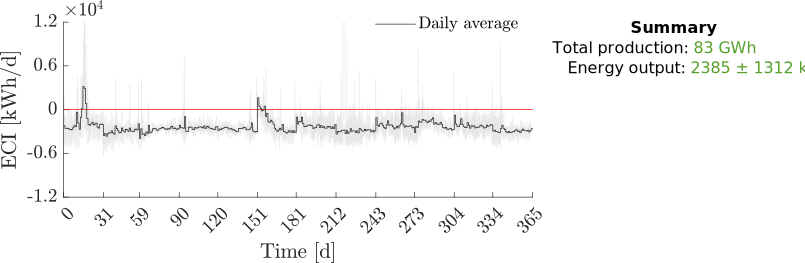
\includegraphics[width=0.85\textwidth]{figs/Simulation_ECI}}%
\end{center}

\end{frame}
%------------------------------------------------------- 
